\input templates/header
\title[DS - Distributed Transactions]{\textbf{Distributed Algorithms}\\Distributed Transactions}

\graphicspath{{figs/14/}}

\newcommand{\RED}[1]{{\small \texttt{\textcolor{darkred}{#1}}}}

\begin{document}

\FrameTitle{Acknowledgement: Diego Ongaro and John Ousterhout}
\FrameContent

%%%%%%%%%%%%%%%%%%%%%%%%%%%%%%%%%%%%%%%%%%%%%%%%%%%%%%%%%%%%%%%%%%%%%%%%%%

\section{Introduction}

\subsection{Motivation}

%-------------------------------------------------------------------------
\begin{frame}{The sad state of Paxos implementations}
\end{frame}


\subsection{Basics}

%-------------------------------------------------------------------------
\begin{frame}{Approaches to Consensus}

Two general approaches to consensus:
\BIL
\item Symmetric, leader-less:
	\BI
	\item All servers have equal roles
	\item Clients can contact any server
	\EI 
\item Asymmetric, leader-based:
	\BI
	\item At any given time, one server is in charge, others accept its decisions
	\item Clients communicate with the leader 
	\EI
\item Raft uses a leader:
	\BI
	\item Decomposes the problem (normal operation, leader changes)
	\item Simplifies normal operation (no conflicts)
	\item More efficient than leader-less approaches
	\EI
\EIL

\end{frame}

\begin{}

%-------------------------------------------------------------------------
\begin{frame}{Raft overview}
	
\BEL
\item Leader election:
	\BI
	\item Select one of the servers to act as leader
	\item Detect crashes, choose new leader
	\EI
\item Normal operation 
	\BI
	\item Basic log replication
	\EI
\item Safety and consistency after leader changes
\item Neutralizing old leaders
\item Client interactions
	\BI
	\item Implementing linearizeable semantics
	\EI
\item Configuration changes
	\BI
	\item Adding and removing servers
	\EI
\EEL

\end{frame}

%-------------------------------------------------------------------------
\begin{frame}{Server states}

\begin{tabular}{| P{2cm} | P{9cm} | }
\hline
\RED{Leader} & Handles all client interactions, log replication \newline
At most 1 viable leader at a time\\\hline
\RED{Follower} & Completely passive (issues no RPCs, responds to incoming RPCs)\\\hline
\RED{Candidate} & Used to elect a new leader\newline
Normal operation: 1 leader, N-1 followers\\\hline
\end{tabular}

\bigskip
\begin{center}
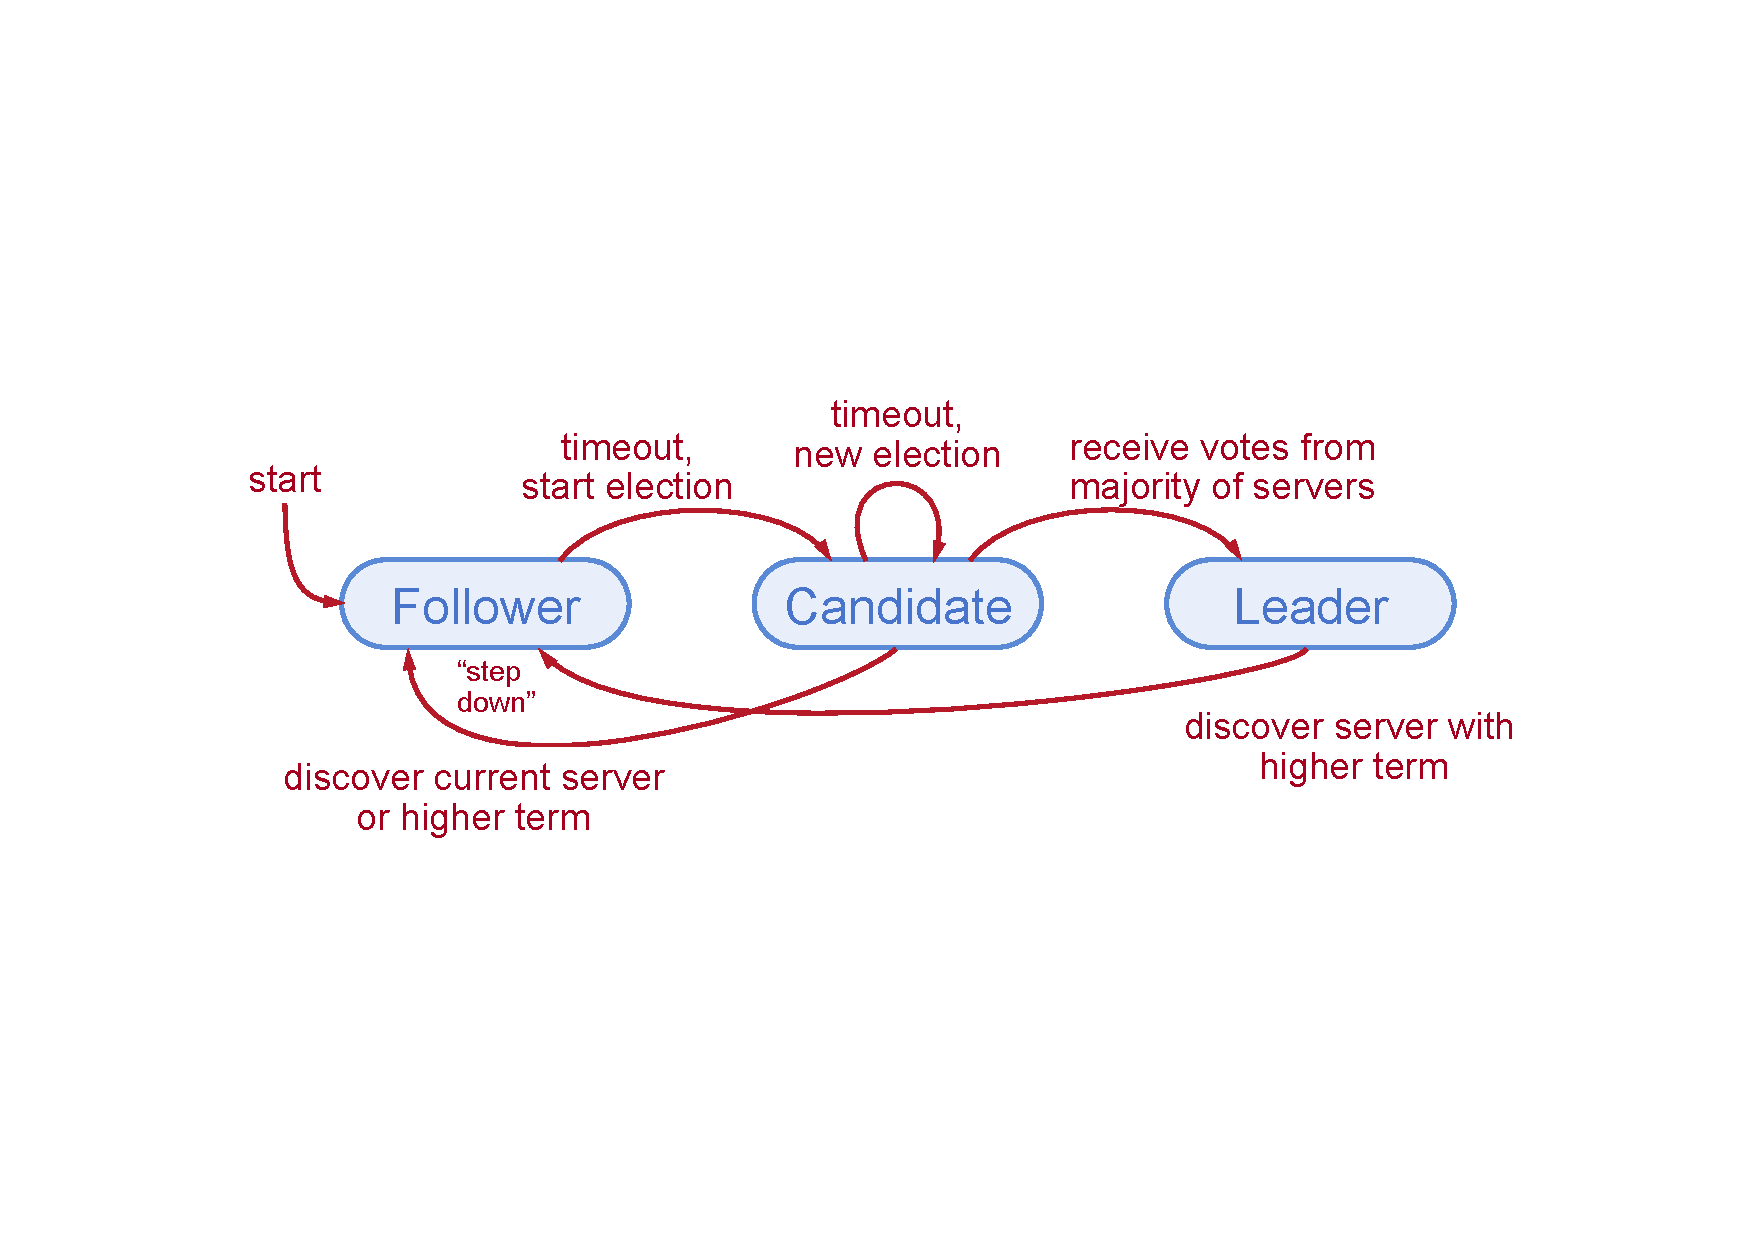
\includegraphics[width=0.90\textwidth]{states.pdf}
\end{center}
\end{frame}

%-------------------------------------------------------------------------
\begin{frame}{Terms}

\begin{center}
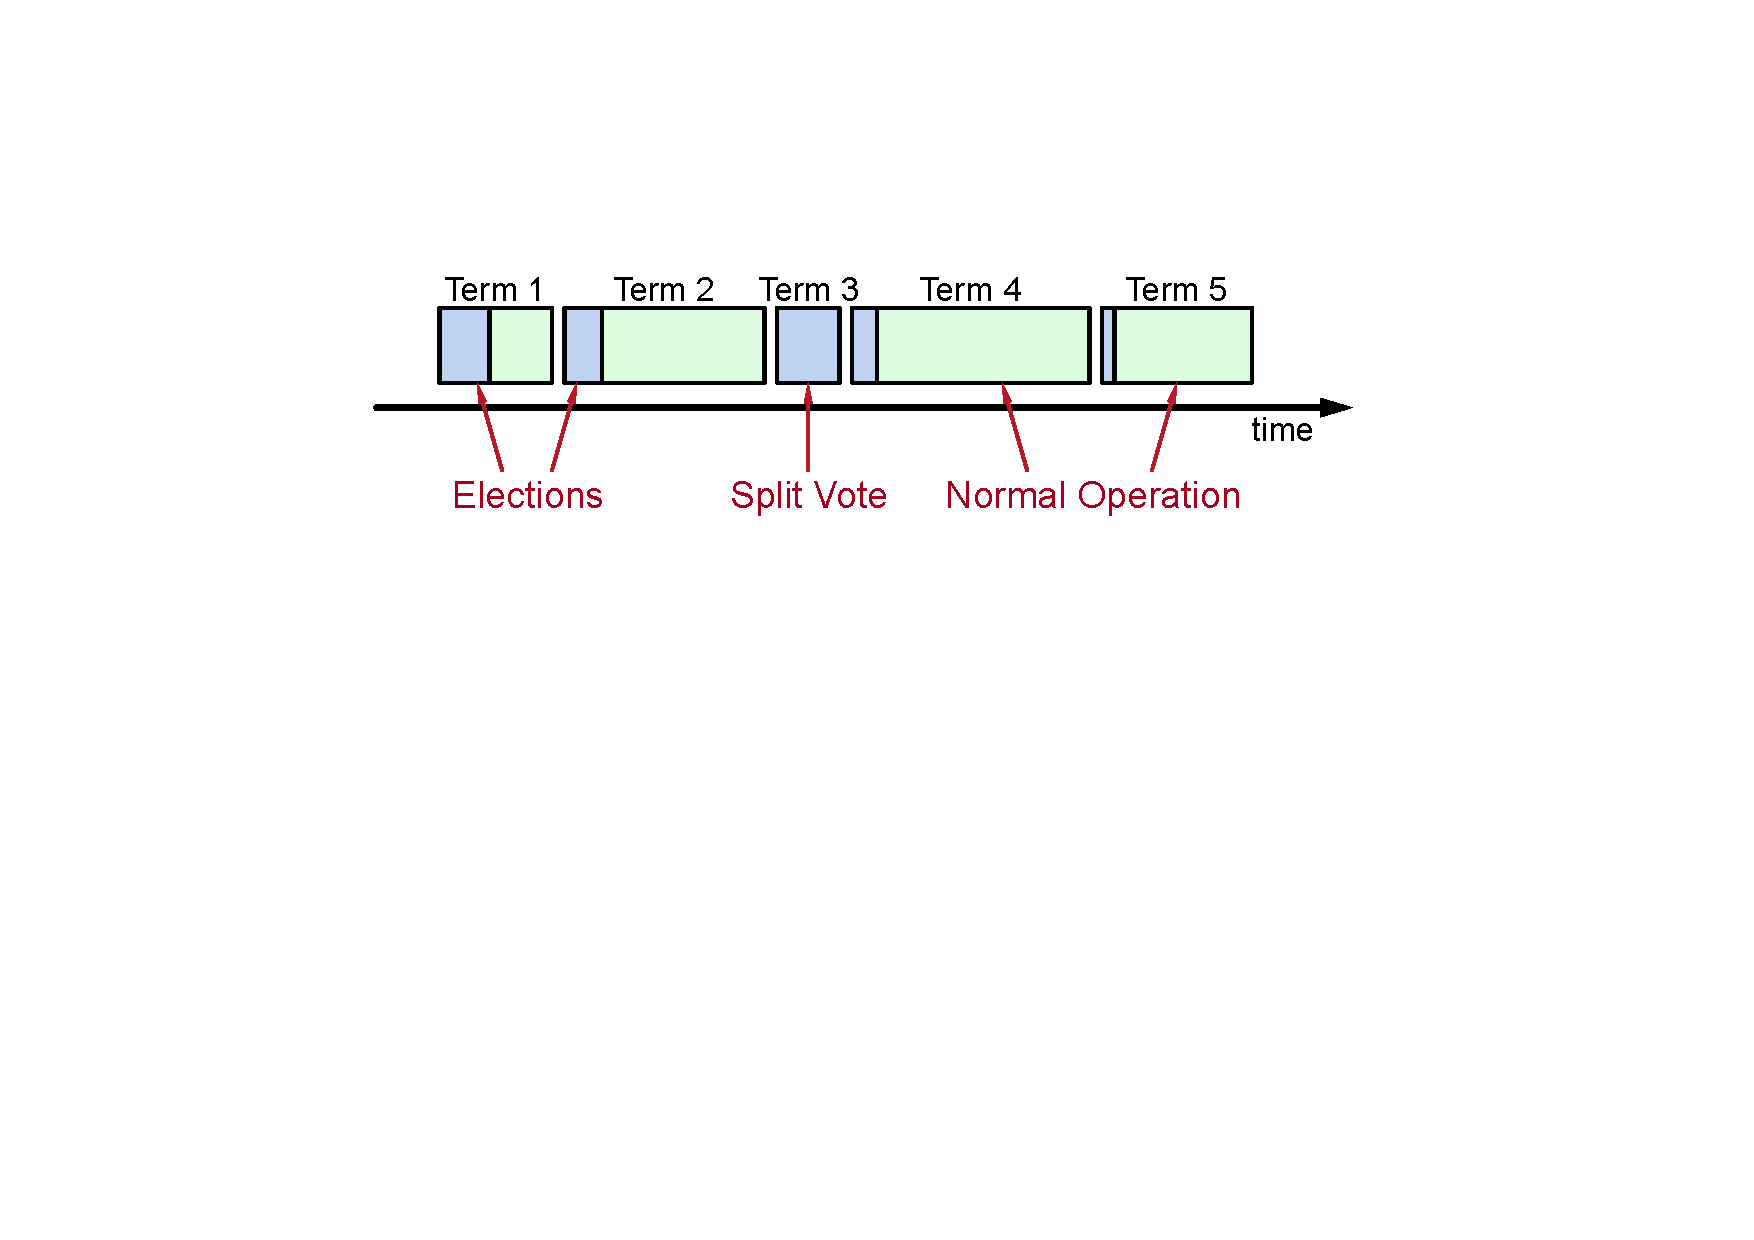
\includegraphics[width=0.70\textwidth]{terms.pdf}
\end{center}

\BIL
\item Time divided into terms:
	\BI
	\item Election
	\item Normal operation under a single leader
	\EI
\item At most 1 leader per term
\item Some terms have no leader (failed election)
\item Each server maintains \alert{current term} value
\item Key role of terms: \alert{identify obsolete information}
\EIL
		
\end{frame}

%-------------------------------------------------------------------------
\begin{frame}{Persistent state}

Each server persists the following to stable storage synchronously before 
responding to RPCs:

\bigskip
\begin{tabular}{| P{2cm} | P{9cm} | }
\hline
\RED{currentTerm}	& Latest term server has seen (initialized to 0 on first boot) \\\hline
\RED{votedFor} & ID of the candidate that received vote in current term (or null if none) \\\hline
\RED{log[]} & Log entries:	

\medskip
\begin{tabular}{| P{1.5cm} | P{6.7cm} | }
\hline
\RED{term} & term when entry was received by leader\\\hline
\RED{index} &	position of entry in the log \\\hline
\RED{command} &	command for state machine \\\hline
\end{tabular}

\\\hline
\end{tabular}

\end{frame}

%-------------------------------------------------------------------------
\begin{frame}{Hearthbeats and timeouts}

\BIL
\item Servers start up as followers
\item Followers expect to receive RPCs from leaders or candidates
\item Leaders must send \alert{heartbeats} (empty \RED{AppendEntries} RPCs) to maintain authority
\item If \RED{electionTimeout} elapses with no RPCs:
	\BI
	\item Follower assumes leader has crashed
	\item Follower starts new election
	\item Timeouts typically 100-500ms
	\EI
\EIL

\end{frame}


%-------------------------------------------------------------------------
\begin{frame}{Election basics}

\BIL
\item Increment current term
\item Change to \RED{Candidate} state
\item Vote for self
\itme Send \RED{RequestVote} RPCs to all other servers, retry until either:
	\BI
	\item Receive votes from majority of servers:
		\BI
		\item Become leader
		\item Send \emph{AppendEntries} heartbeats to all other servers
		\EI
	\item Receive RPC from valid leader:
		\BI
		\item Return to follower state
		\EI
	\item No-one wins election (election timeout elapses):
		\BI
		\item Increment term, start new election
		\EI
	\EI
\EIL

\end{frame}

%-------------------------------------------------------------------------
\begin{frame}{}
\end{frame}


%-------------------------------------------------------------------------
\begin{RMFrame}

\BI
\item \bibentry{raft}
\EI

\end{RMFrame}


\end{document}

%-------------------------------------------------------------------------
\begin{frame}{}
\end{frame}
